\documentclass[tikz,border=0mm]{standalone}
\usepackage[T1]{fontenc}
\usepackage{lmodern,amsmath,pgfplots}
\usetikzlibrary{arrows.meta}
\pgfplotsset{compat=1.18}

\definecolor{Ink}{HTML}{173047}
\definecolor{Navy}{HTML}{17486F}
\definecolor{Blue}{HTML}{377797}
\definecolor{Slate}{HTML}{526D80}
\definecolor{Guide}{HTML}{8A9EAD}
\definecolor{Grid}{HTML}{DCE5EA}
\definecolor{Pale}{HTML}{E8F0F5}

% Theorem 1 witness and the tau=0.5, eta=0.2 record in direct_witness.json.
\def\CapMagnitude{4}
\def\InitSpeed{25}
\def\TargetFraction{0.9}
\def\SharedTiming{0.9}
\def\ShortRamp{0.2}
\def\MiddleRamp{0.5}
\def\LongRamp{0.8}
\def\SampleTime{0.81}
\def\Report{2.88}
\def\ErrorWidth{0.20}
\def\Reserve{2}
\def\LeadCap{6}
\def\LeadLag{0.1}
\def\LeadRamp{0.6}

\tikzset{
  short ramp/.style={draw=Navy,line width=1pt},
  middle ramp/.style={draw=Blue,line width=1.05pt,dash pattern=on 3.6pt off 1.85pt},
  long ramp/.style={draw=Slate,line width=1.1pt,dash pattern=on .45pt off 1.7pt},
  title text/.style={anchor=west,inner sep=0pt,font=\sffamily\bfseries\fontsize{10.3}{12}\selectfont},
  left text/.style={anchor=west,inner sep=0pt},
  right text/.style={anchor=east,inner sep=0pt},
  declare function={
    rampstart(\d)=\SharedTiming-\TargetFraction*\d;
    rampelapsed(\t,\d)=min(max(\t-rampstart(\d),0),\d);
    plateauelapsed(\t,\d)=max(0,\t-rampstart(\d)-\d);
    cappedelapsed(\t,\d)=min(plateauelapsed(\t,\d),\InitSpeed/\CapMagnitude-\d/2);
    rampspeed(\t,\d)=max(0,\InitSpeed-\CapMagnitude*(rampelapsed(\t,\d)^2/(2*\d)+plateauelapsed(\t,\d)));
    ramptravel(\t,\d)=\InitSpeed*min(\t,rampstart(\d))+\InitSpeed*rampelapsed(\t,\d)
      -\CapMagnitude*rampelapsed(\t,\d)^3/(6*\d)+(\InitSpeed-\CapMagnitude*\d/2)*cappedelapsed(\t,\d)
      -\CapMagnitude*cappedelapsed(\t,\d)^2/2;
    stopdist(\d)=\InitSpeed*\SharedTiming+\InitSpeed^2/(2*\CapMagnitude)
      +\InitSpeed*(0.5-\TargetFraction)*\d-\CapMagnitude*\d^2/24;
  }
}
\pgfplotsset{
  manuscript axis/.style={
    scale only axis,anchor=south west,axis x line*=bottom,axis y line*=left,
    axis line style={draw=Slate,line width=.55pt},
    tick style={draw=Slate,line width=.45pt},major tick length=1.8pt,
    tick align=outside,scaled ticks=false,ymajorgrids=true,
    grid style={draw=Grid,line width=.38pt},enlargelimits=false,
    tick label style={font=\sffamily\fontsize{8.7}{10}\selectfont,text=Ink},
    label style={font=\sffamily\fontsize{9.1}{11}\selectfont,text=Ink},
    every axis x label/.append style={at={(axis description cs:0.5,0)},yshift=-5.4mm,anchor=north,inner sep=0pt},
    every axis y label/.append style={inner sep=1pt}
  }
}

% The onset, common 90% point, and plateau start are explicit plot vertices.
\newcommand{\DrawMagnitude}[2]{%
  \pgfmathsetmacro{\onset}{\SharedTiming-\TargetFraction*#2}%
  \pgfmathsetmacro{\plateau}{\onset+#2}%
  \addplot[#1,no marks] coordinates {
    (0,0) (\onset,0) (\SharedTiming,\sharedMagnitude) (\plateau,\CapMagnitude) (1.2,\CapMagnitude)
  };%
}
\newcommand{\TruckIcon}[2]{%
  \begin{scope}[shift={(#1,#2)},line width=.65pt]
    \filldraw[fill=Pale,draw=Navy] (-10,2) rectangle (4.2,7.8);
    \filldraw[fill=Grid,draw=Navy] (4.2,2) -- (4.2,6.7) -- (7.8,6.7)
      -- (10.2,4.6) -- (10.2,2) -- cycle;
    \draw[draw=Navy,line width=.45pt] (5.4,6.4) -- (5.4,4.5) -- (9.85,4.5);
    \fill[Navy] (-6.5,1.15) circle[radius=1.25mm] (7.5,1.15) circle[radius=1.25mm];
    \fill[white] (-6.5,1.15) circle[radius=.40mm] (7.5,1.15) circle[radius=.40mm];
  \end{scope}%
}
\newcommand{\GapNumber}[1]{\pgfmathprintnumber[fixed,fixed zerofill,precision=3]{#1}}
\newcommand{\GapBar}[4]{%
  \draw[draw=#4,line width=2.65pt] ({85+10*(#1-32)},#3) -- ({85+10*(#2-32)},#3);
  \fill[#4] ({85+10*(#1-32)},#3) circle[radius=1.04mm];
  \fill[#4] ({85+10*(#2-32)},#3) circle[radius=1.04mm];
}

\begin{document}
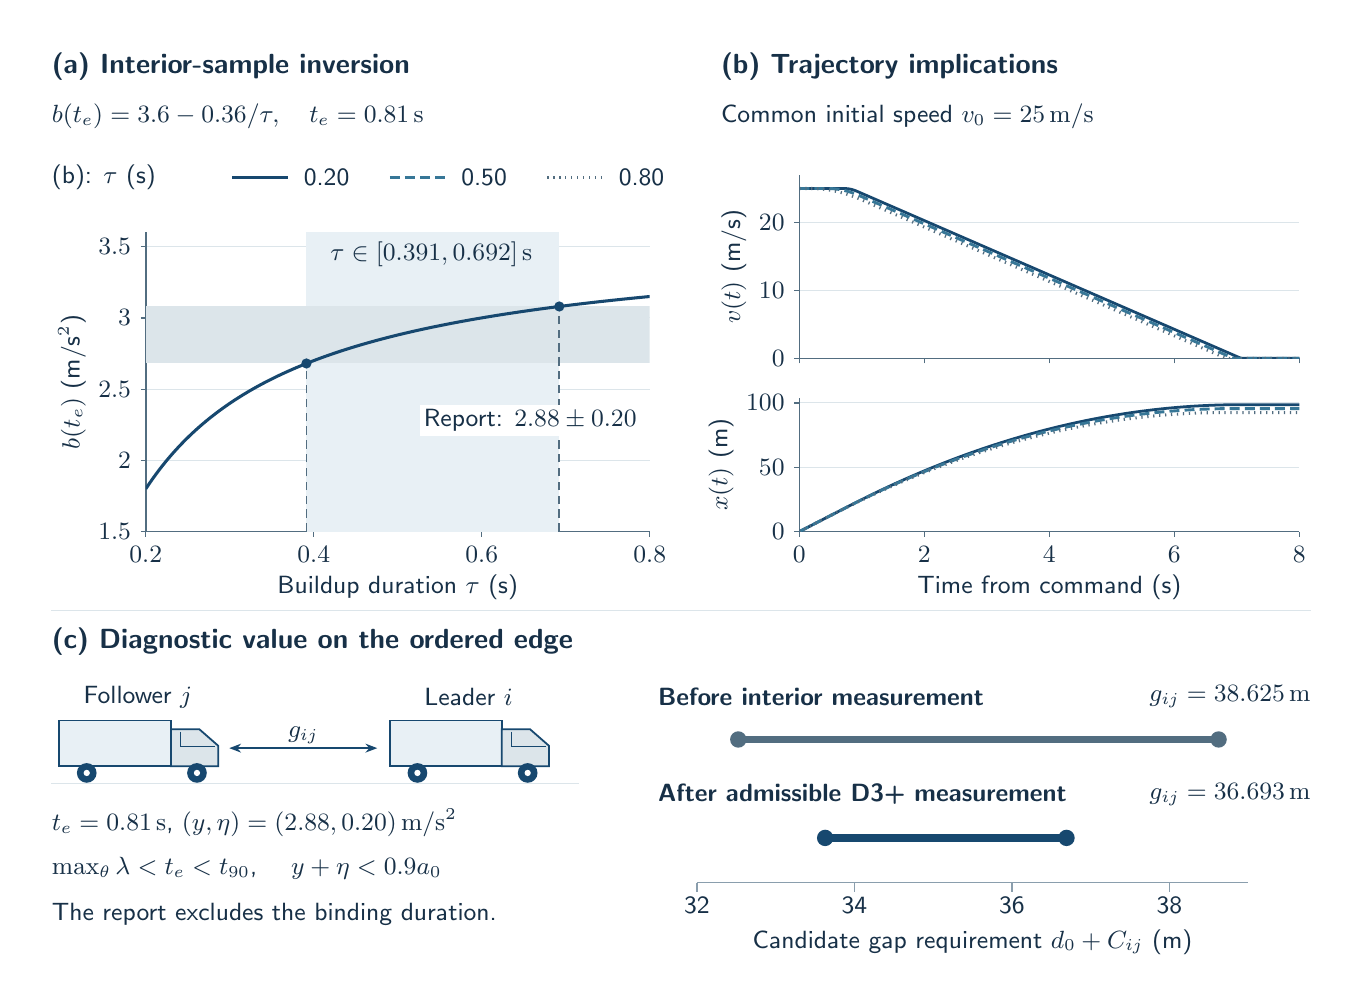
\begin{tikzpicture}[x=1mm,y=1mm,text=Ink,font=\sffamily\fontsize{9.1}{11}\selectfont]
\path[use as bounding box] (0,0) rectangle (166,119);
\fill[white] (0,0) rectangle (166,119);
\pgfmathsetmacro{\sharedMagnitude}{\CapMagnitude*\TargetFraction}
\pgfmathsetmacro{\featureLow}{\Report-\ErrorWidth}
\pgfmathsetmacro{\featureHigh}{\Report+\ErrorWidth}
\pgfmathsetmacro{\capLeft}{\SampleTime-0.015}
\pgfmathsetmacro{\capRight}{\SampleTime+0.015}

\pgfmathsetmacro{\postLow}{max(\ShortRamp,\CapMagnitude*(\SharedTiming-\SampleTime)/(\CapMagnitude*\TargetFraction-\Report+\ErrorWidth))}
\pgfmathsetmacro{\postHigh}{min(\LongRamp,\CapMagnitude*(\SharedTiming-\SampleTime)/(\CapMagnitude*\TargetFraction-\Report-\ErrorWidth))}

\node[title text] at (3,114) {(a) Interior-sample inversion};
\node[left text] at (3,107.7) {\(b(t_e)=3.6-0.36/\tau,\quad t_e=0.81\,\mathrm{s}\)};
\node[left text] at (3,100) {(b): \(\tau\) (s)};
\draw[short ramp] (26,100) -- (33,100);
\node[left text] at (35,100) {0.20};
\draw[middle ramp] (46,100) -- (53,100);
\node[left text] at (55,100) {0.50};
\draw[long ramp] (66,100) -- (73,100);
\node[left text] at (75,100) {0.80};
\begin{axis}[
  manuscript axis,at={(15mm,55mm)},width=64mm,height=38mm,
  xmin=0.2,xmax=0.8,ymin=1.5,ymax=3.6,
  xtick={0.2,0.4,0.6,0.8},ytick={1.5,2,2.5,3,3.5},
  xlabel={Buildup duration \(\tau\) (s)},ylabel={\(b(t_e)\) (m/s\(^2\))}
]
  \path[fill=Pale] (axis cs:\postLow,1.5) rectangle (axis cs:\postHigh,3.6);
  \path[fill=Grid] (axis cs:.2,\featureLow) rectangle (axis cs:.8,\featureHigh);
  \addplot[draw=Navy,line width=1.1pt,domain=.2:.8,samples=151]
    {\CapMagnitude*(\TargetFraction-(\SharedTiming-\SampleTime)/x)};
  \draw[draw=Slate,densely dashed,line width=.6pt]
    (axis cs:\postLow,1.5) -- (axis cs:\postLow,\featureLow)
    (axis cs:\postHigh,1.5) -- (axis cs:\postHigh,\featureHigh);
  \fill[Navy] (axis cs:\postLow,\featureLow) circle[radius=.65mm]
    (axis cs:\postHigh,\featureHigh) circle[radius=.65mm];
  \node[anchor=north,inner sep=1pt,font=\sffamily\fontsize{8.7}{10}\selectfont]
    at (axis cs:.54,3.56) {\(\tau\in[0.391,0.692]\,\mathrm{s}\)};
  \node[anchor=south east,inner sep=1.5pt,fill=white,font=\sffamily\fontsize{8.7}{10}\selectfont]
    at (axis cs:.79,2.17) {Report: \(2.88\pm0.20\)};
\end{axis}

\node[title text] at (88,114) {(b) Trajectory implications};
\node[left text] at (88,107.7) {Common initial speed \(v_0=25\,\mathrm{m/s}\)};
\begin{axis}[
  manuscript axis,at={(98mm,77mm)},width=63.5mm,height=23.3mm,
  xmin=0,xmax=8,ymin=0,ymax=27,xtick={0,2,4,6,8},xticklabels=\empty,
  ytick={0,10,20},ylabel={\(v(t)\) (m/s)},domain=0:8,samples=241
]
  \addplot[short ramp] {rampspeed(x,\ShortRamp)};
  \addplot[middle ramp] {rampspeed(x,\MiddleRamp)};
  \addplot[long ramp] {rampspeed(x,\LongRamp)};
\end{axis}
\begin{axis}[
  manuscript axis,at={(98mm,55mm)},width=63.5mm,height=17mm,
  xmin=0,xmax=8,ymin=0,ymax=104,xtick={0,2,4,6,8},ytick={0,50,100},
  xlabel={Time from command (s)},ylabel={\(x(t)\) (m)},domain=0:8,samples=241
]
  \addplot[short ramp] {ramptravel(x,\ShortRamp)};
  \addplot[middle ramp] {ramptravel(x,\MiddleRamp)};
  \addplot[long ramp] {ramptravel(x,\LongRamp)};
\end{axis}

\draw[draw=Grid,line width=.6pt] (3,45) -- (163,45);
\node[title text] at (3,41) {(c) Diagnostic value on the ordered edge};
\draw[draw=Grid,line width=.6pt] (3,23) -- (70,23);
\TruckIcon{14}{23.2}
\TruckIcon{56}{23.2}
\node[inner sep=0pt] at (14,34) {Follower \(j\)};
\node[inner sep=0pt] at (56,34) {Leader \(i\)};
\draw[draw=Navy,line width=.65pt,{Stealth[length=1.5mm]}-{Stealth[length=1.5mm]}]
  (25.6,27.5) -- node[above,inner sep=1.2pt] {\(g_{ij}\)} (44.4,27.5);
\node[left text] at (3,18) {\(t_e=0.81\,\mathrm{s}\), \((y,\eta)=(2.88,0.20)\,\mathrm{m/s^2}\)};
\node[left text] at (3,12.2) {\(\max_\theta\lambda<t_e<t_{90}\), \quad \(y+\eta<0.9a_0\)};
\node[left text] at (3,6.4) {The report excludes the binding duration.};

% Equation (9) gives the intersection. Equation (6) is decreasing in tau
% on this support, and closure is the stopping-distance difference.
\pgfmathsetmacro{\postlow}{max(\ShortRamp, \CapMagnitude*(\SharedTiming-\SampleTime)/(\CapMagnitude*\TargetFraction-\Report+\ErrorWidth))}
\pgfmathsetmacro{\posthigh}{min(\LongRamp, \CapMagnitude*(\SharedTiming-\SampleTime)/(\CapMagnitude*\TargetFraction-\Report-\ErrorWidth))}
\pgfmathsetmacro{\leadstop}{\InitSpeed*\LeadLag+\InitSpeed*\LeadRamp/2+\InitSpeed^2/(2*\LeadCap)-\LeadCap*\LeadRamp^2/24}
\pgfmathsetmacro{\gBeforeMin}{\Reserve+stopdist(\LongRamp)-\leadstop}
\pgfmathsetmacro{\gBeforeMax}{\Reserve+stopdist(\ShortRamp)-\leadstop}
\pgfmathsetmacro{\gAfterMin}{\Reserve+stopdist(\posthigh)-\leadstop}
\pgfmathsetmacro{\gAfterMax}{\Reserve+stopdist(\postlow)-\leadstop}
\node[left text,font=\sffamily\bfseries\fontsize{9.1}{11}\selectfont] at (80,34) {Before interior measurement};
\node[right text] at (163,34) {\(g_{ij}=\GapNumber{\gBeforeMax}\,\mathrm{m}\)};
\GapBar{\gBeforeMin}{\gBeforeMax}{28.6}{Slate}
\node[left text,font=\sffamily\bfseries\fontsize{9.1}{11}\selectfont] at (80,21.6) {After admissible D3+ measurement};
\node[right text] at (163,21.6) {\(g_{ij}=\GapNumber{\gAfterMax}\,\mathrm{m}\)};
\GapBar{\gAfterMin}{\gAfterMax}{16.1}{Navy}
\draw[draw=Guide,line width=.45pt] (85,10.4) -- (155,10.4);
\foreach \m in {32,34,36,38}{
  \draw[draw=Guide,line width=.45pt] ({85+10*(\m-32)},10.4) -- ++(0,-1.2);
  \node[anchor=north,inner sep=0pt] at ({85+10*(\m-32)},8.6) {\m};
}
\node[inner sep=0pt] at (120,2.9) {Candidate gap requirement \(d_0+C_{ij}\) (m)};
\end{tikzpicture}
\end{document}
